% Options for packages loaded elsewhere
\PassOptionsToPackage{unicode}{hyperref}
\PassOptionsToPackage{hyphens}{url}
%
\documentclass[
]{article}
\usepackage{amsmath,amssymb}
\usepackage{iftex}
\ifPDFTeX
  \usepackage[T1]{fontenc}
  \usepackage[utf8]{inputenc}
  \usepackage{textcomp} % provide euro and other symbols
\else % if luatex or xetex
  \usepackage{unicode-math} % this also loads fontspec
  \defaultfontfeatures{Scale=MatchLowercase}
  \defaultfontfeatures[\rmfamily]{Ligatures=TeX,Scale=1}
\fi
\usepackage{lmodern}
\ifPDFTeX\else
  % xetex/luatex font selection
\fi
% Use upquote if available, for straight quotes in verbatim environments
\IfFileExists{upquote.sty}{\usepackage{upquote}}{}
\IfFileExists{microtype.sty}{% use microtype if available
  \usepackage[]{microtype}
  \UseMicrotypeSet[protrusion]{basicmath} % disable protrusion for tt fonts
}{}
\makeatletter
\@ifundefined{KOMAClassName}{% if non-KOMA class
  \IfFileExists{parskip.sty}{%
    \usepackage{parskip}
  }{% else
    \setlength{\parindent}{0pt}
    \setlength{\parskip}{6pt plus 2pt minus 1pt}}
}{% if KOMA class
  \KOMAoptions{parskip=half}}
\makeatother
\usepackage{xcolor}
\usepackage[margin=1in]{geometry}
\usepackage{color}
\usepackage{fancyvrb}
\newcommand{\VerbBar}{|}
\newcommand{\VERB}{\Verb[commandchars=\\\{\}]}
\DefineVerbatimEnvironment{Highlighting}{Verbatim}{commandchars=\\\{\}}
% Add ',fontsize=\small' for more characters per line
\usepackage{framed}
\definecolor{shadecolor}{RGB}{248,248,248}
\newenvironment{Shaded}{\begin{snugshade}}{\end{snugshade}}
\newcommand{\AlertTok}[1]{\textcolor[rgb]{0.94,0.16,0.16}{#1}}
\newcommand{\AnnotationTok}[1]{\textcolor[rgb]{0.56,0.35,0.01}{\textbf{\textit{#1}}}}
\newcommand{\AttributeTok}[1]{\textcolor[rgb]{0.13,0.29,0.53}{#1}}
\newcommand{\BaseNTok}[1]{\textcolor[rgb]{0.00,0.00,0.81}{#1}}
\newcommand{\BuiltInTok}[1]{#1}
\newcommand{\CharTok}[1]{\textcolor[rgb]{0.31,0.60,0.02}{#1}}
\newcommand{\CommentTok}[1]{\textcolor[rgb]{0.56,0.35,0.01}{\textit{#1}}}
\newcommand{\CommentVarTok}[1]{\textcolor[rgb]{0.56,0.35,0.01}{\textbf{\textit{#1}}}}
\newcommand{\ConstantTok}[1]{\textcolor[rgb]{0.56,0.35,0.01}{#1}}
\newcommand{\ControlFlowTok}[1]{\textcolor[rgb]{0.13,0.29,0.53}{\textbf{#1}}}
\newcommand{\DataTypeTok}[1]{\textcolor[rgb]{0.13,0.29,0.53}{#1}}
\newcommand{\DecValTok}[1]{\textcolor[rgb]{0.00,0.00,0.81}{#1}}
\newcommand{\DocumentationTok}[1]{\textcolor[rgb]{0.56,0.35,0.01}{\textbf{\textit{#1}}}}
\newcommand{\ErrorTok}[1]{\textcolor[rgb]{0.64,0.00,0.00}{\textbf{#1}}}
\newcommand{\ExtensionTok}[1]{#1}
\newcommand{\FloatTok}[1]{\textcolor[rgb]{0.00,0.00,0.81}{#1}}
\newcommand{\FunctionTok}[1]{\textcolor[rgb]{0.13,0.29,0.53}{\textbf{#1}}}
\newcommand{\ImportTok}[1]{#1}
\newcommand{\InformationTok}[1]{\textcolor[rgb]{0.56,0.35,0.01}{\textbf{\textit{#1}}}}
\newcommand{\KeywordTok}[1]{\textcolor[rgb]{0.13,0.29,0.53}{\textbf{#1}}}
\newcommand{\NormalTok}[1]{#1}
\newcommand{\OperatorTok}[1]{\textcolor[rgb]{0.81,0.36,0.00}{\textbf{#1}}}
\newcommand{\OtherTok}[1]{\textcolor[rgb]{0.56,0.35,0.01}{#1}}
\newcommand{\PreprocessorTok}[1]{\textcolor[rgb]{0.56,0.35,0.01}{\textit{#1}}}
\newcommand{\RegionMarkerTok}[1]{#1}
\newcommand{\SpecialCharTok}[1]{\textcolor[rgb]{0.81,0.36,0.00}{\textbf{#1}}}
\newcommand{\SpecialStringTok}[1]{\textcolor[rgb]{0.31,0.60,0.02}{#1}}
\newcommand{\StringTok}[1]{\textcolor[rgb]{0.31,0.60,0.02}{#1}}
\newcommand{\VariableTok}[1]{\textcolor[rgb]{0.00,0.00,0.00}{#1}}
\newcommand{\VerbatimStringTok}[1]{\textcolor[rgb]{0.31,0.60,0.02}{#1}}
\newcommand{\WarningTok}[1]{\textcolor[rgb]{0.56,0.35,0.01}{\textbf{\textit{#1}}}}
\usepackage{graphicx}
\makeatletter
\def\maxwidth{\ifdim\Gin@nat@width>\linewidth\linewidth\else\Gin@nat@width\fi}
\def\maxheight{\ifdim\Gin@nat@height>\textheight\textheight\else\Gin@nat@height\fi}
\makeatother
% Scale images if necessary, so that they will not overflow the page
% margins by default, and it is still possible to overwrite the defaults
% using explicit options in \includegraphics[width, height, ...]{}
\setkeys{Gin}{width=\maxwidth,height=\maxheight,keepaspectratio}
% Set default figure placement to htbp
\makeatletter
\def\fps@figure{htbp}
\makeatother
\setlength{\emergencystretch}{3em} % prevent overfull lines
\providecommand{\tightlist}{%
  \setlength{\itemsep}{0pt}\setlength{\parskip}{0pt}}
\setcounter{secnumdepth}{5}
\ifLuaTeX
  \usepackage{selnolig}  % disable illegal ligatures
\fi
\IfFileExists{bookmark.sty}{\usepackage{bookmark}}{\usepackage{hyperref}}
\IfFileExists{xurl.sty}{\usepackage{xurl}}{} % add URL line breaks if available
\urlstyle{same}
\hypersetup{
  pdftitle={Do ESG Scores Reflect Real Environmental Impact?},
  pdfauthor={Nelly Nie},
  hidelinks,
  pdfcreator={LaTeX via pandoc}}

\title{Do ESG Scores Reflect Real Environmental Impact?}
\author{Nelly Nie}
\date{}

\begin{document}
\maketitle

{
\setcounter{tocdepth}{2}
\tableofcontents
}
\#\#Introduction This analysis investigates whether ESG environmental
scores correlate with actual CO₂ emissions. Using company-level ESG
ratings and historical emissions data, we assess the strength and
significance of this relationship, focusing especially on firms with
high emissions exposure.

\begin{Shaded}
\begin{Highlighting}[]
\FunctionTok{library}\NormalTok{(tidyverse)}
\end{Highlighting}
\end{Shaded}

\begin{verbatim}
## -- Attaching core tidyverse packages ------------------------ tidyverse 2.0.0 --
## v dplyr     1.1.4     v readr     2.1.5
## v forcats   1.0.0     v stringr   1.5.1
## v ggplot2   3.5.2     v tibble    3.2.1
## v lubridate 1.9.3     v tidyr     1.3.1
## v purrr     1.0.2     
## -- Conflicts ------------------------------------------ tidyverse_conflicts() --
## x dplyr::filter() masks stats::filter()
## x dplyr::lag()    masks stats::lag()
## i Use the conflicted package (<http://conflicted.r-lib.org/>) to force all conflicts to become errors
\end{verbatim}

\begin{Shaded}
\begin{Highlighting}[]
\FunctionTok{library}\NormalTok{(readr)}
\FunctionTok{library}\NormalTok{(fuzzyjoin)}
\FunctionTok{library}\NormalTok{(dplyr)}
\FunctionTok{library}\NormalTok{(ggplot2)}
\FunctionTok{library}\NormalTok{(stringdist)}
\end{Highlighting}
\end{Shaded}

\begin{verbatim}
## 
## Attaching package: 'stringdist'
## 
## The following object is masked from 'package:tidyr':
## 
##     extract
\end{verbatim}

\#\#1.Load Data

\begin{Shaded}
\begin{Highlighting}[]
\NormalTok{esg\_data }\OtherTok{\textless{}{-}} \FunctionTok{read\_csv}\NormalTok{(}\StringTok{"data/data.csv"}\NormalTok{)}
\end{Highlighting}
\end{Shaded}

\begin{verbatim}
## Rows: 722 Columns: 21
## -- Column specification --------------------------------------------------------
## Delimiter: ","
## chr (16): ticker, name, currency, exchange, industry, logo, weburl, environm...
## dbl  (5): environment_score, social_score, governance_score, total_score, cik
## 
## i Use `spec()` to retrieve the full column specification for this data.
## i Specify the column types or set `show_col_types = FALSE` to quiet this message.
\end{verbatim}

\begin{Shaded}
\begin{Highlighting}[]
\NormalTok{emissions }\OtherTok{\textless{}{-}} \FunctionTok{read\_csv}\NormalTok{(}\StringTok{"data/emissions\_medium\_granularity.csv"}\NormalTok{)}
\end{Highlighting}
\end{Shaded}

\begin{verbatim}
## Rows: 12551 Columns: 7
## -- Column specification --------------------------------------------------------
## Delimiter: ","
## chr (4): parent_entity, parent_type, commodity, production_unit
## dbl (3): year, production_value, total_emissions_MtCO2e
## 
## i Use `spec()` to retrieve the full column specification for this data.
## i Specify the column types or set `show_col_types = FALSE` to quiet this message.
\end{verbatim}

\hypertarget{data-cleaning-preparation}{%
\subsection{2. Data Cleaning \&
Preparation}\label{data-cleaning-preparation}}

\begin{Shaded}
\begin{Highlighting}[]
\CommentTok{\# Step 1: Filter irrelevant data }
\NormalTok{esg\_clean }\OtherTok{\textless{}{-}}\NormalTok{ esg\_data }\SpecialCharTok{\%\textgreater{}\%}
  \FunctionTok{select}\NormalTok{(name, ticker, industry, environment\_score, social\_score, governance\_score, total\_score, total\_grade) }\SpecialCharTok{\%\textgreater{}\%}
  \FunctionTok{filter}\NormalTok{(}\SpecialCharTok{!}\FunctionTok{is.na}\NormalTok{(environment\_score))}

\NormalTok{emissions\_latest }\OtherTok{\textless{}{-}}\NormalTok{ emissions }\SpecialCharTok{\%\textgreater{}\%}
  \FunctionTok{group\_by}\NormalTok{(parent\_entity) }\SpecialCharTok{\%\textgreater{}\%}
  \FunctionTok{filter}\NormalTok{(year }\SpecialCharTok{==} \FunctionTok{max}\NormalTok{(year)) }\SpecialCharTok{\%\textgreater{}\%}
  \FunctionTok{summarise}\NormalTok{(}\AttributeTok{total\_emissions =} \FunctionTok{sum}\NormalTok{(total\_emissions\_MtCO2e, }\AttributeTok{na.rm =} \ConstantTok{TRUE}\NormalTok{)) }\SpecialCharTok{\%\textgreater{}\%}
  \FunctionTok{ungroup}\NormalTok{()}
\end{Highlighting}
\end{Shaded}

\begin{Shaded}
\begin{Highlighting}[]
\CommentTok{\# Step 2: Remove duplicates by choosing closest match}
\NormalTok{fuzzy\_merged }\OtherTok{\textless{}{-}} \FunctionTok{stringdist\_left\_join}\NormalTok{(}
\NormalTok{  esg\_clean,}
\NormalTok{  emissions\_latest,}
  \AttributeTok{by =} \FunctionTok{c}\NormalTok{(}\StringTok{"name"} \OtherTok{=} \StringTok{"parent\_entity"}\NormalTok{),}
  \AttributeTok{method =} \StringTok{"jw"}\NormalTok{,}
  \AttributeTok{max\_dist =} \FloatTok{0.25}
\NormalTok{)}

\NormalTok{fuzzy\_merged\_clean }\OtherTok{\textless{}{-}}\NormalTok{ fuzzy\_merged }\SpecialCharTok{\%\textgreater{}\%}
  \FunctionTok{mutate}\NormalTok{(}\AttributeTok{dist =} \FunctionTok{stringdist}\NormalTok{(name, parent\_entity, }\AttributeTok{method =} \StringTok{"jw"}\NormalTok{)) }\SpecialCharTok{\%\textgreater{}\%}
  \FunctionTok{group\_by}\NormalTok{(name) }\SpecialCharTok{\%\textgreater{}\%}
  \FunctionTok{slice\_min}\NormalTok{(}\AttributeTok{order\_by =}\NormalTok{ dist, }\AttributeTok{n =} \DecValTok{1}\NormalTok{) }\SpecialCharTok{\%\textgreater{}\%}
  \FunctionTok{ungroup}\NormalTok{() }\SpecialCharTok{\%\textgreater{}\%}
  \FunctionTok{select}\NormalTok{(}\SpecialCharTok{{-}}\NormalTok{dist)  }\CommentTok{\# optional cleanup}
\end{Highlighting}
\end{Shaded}

\begin{Shaded}
\begin{Highlighting}[]
\CommentTok{\# Step 3: Check for successful matches}
\FunctionTok{summary}\NormalTok{(fuzzy\_merged\_clean}\SpecialCharTok{$}\NormalTok{total\_emissions)}
\end{Highlighting}
\end{Shaded}

\begin{verbatim}
##     Min.  1st Qu.   Median     Mean  3rd Qu.     Max.     NA's 
##    11.34    51.41    98.81   634.84   172.56 12290.38      697
\end{verbatim}

\begin{Shaded}
\begin{Highlighting}[]
\FunctionTok{glimpse}\NormalTok{(fuzzy\_merged\_clean)}
\end{Highlighting}
\end{Shaded}

\begin{verbatim}
## Rows: 722
## Columns: 10
## $ name              <chr> "3M Co", "A O Smith Corp", "ABIOMED Inc", "ABVC Biop~
## $ ticker            <chr> "mmm", "aos", "abmd", "abvc", "aciu", "acad", "acev"~
## $ industry          <chr> "Industrial Conglomerates", "Building", "Health Care~
## $ environment_score <dbl> 526, 510, 500, 220, 250, 230, 225, 500, 410, 220, 23~
## $ social_score      <dbl> 310, 315, 324, 212, 296, 230, 211, 327, 232, 219, 26~
## $ governance_score  <dbl> 305, 310, 305, 205, 305, 305, 215, 300, 325, 215, 31~
## $ total_score       <dbl> 1141, 1135, 1129, 637, 851, 765, 651, 1127, 967, 654~
## $ total_grade       <chr> "BBB", "BBB", "BBB", "B", "BB", "BB", "B", "BBB", "B~
## $ parent_entity     <chr> NA, NA, NA, NA, NA, NA, NA, NA, NA, NA, NA, NA, NA, ~
## $ total_emissions   <dbl> NA, NA, NA, NA, NA, NA, NA, NA, NA, NA, NA, NA, NA, ~
\end{verbatim}

\begin{Shaded}
\begin{Highlighting}[]
\CommentTok{\# Check if any company name still has \textgreater{}1 match}
\NormalTok{fuzzy\_merged\_clean }\SpecialCharTok{\%\textgreater{}\%}
  \FunctionTok{count}\NormalTok{(name) }\SpecialCharTok{\%\textgreater{}\%}
  \FunctionTok{filter}\NormalTok{(n }\SpecialCharTok{\textgreater{}} \DecValTok{1}\NormalTok{)}
\end{Highlighting}
\end{Shaded}

\begin{verbatim}
## # A tibble: 0 x 2
## # i 2 variables: name <chr>, n <int>
\end{verbatim}

\begin{Shaded}
\begin{Highlighting}[]
\NormalTok{fuzzy\_merged\_clean }\SpecialCharTok{\%\textgreater{}\%}
  \FunctionTok{filter}\NormalTok{(}\SpecialCharTok{!}\FunctionTok{is.na}\NormalTok{(total\_emissions)) }\SpecialCharTok{\%\textgreater{}\%}
  \FunctionTok{select}\NormalTok{(name, parent\_entity, total\_emissions)}
\end{Highlighting}
\end{Shaded}

\begin{verbatim}
## # A tibble: 25 x 3
##    name                   parent_entity  total_emissions
##    <chr>                  <chr>                    <dbl>
##  1 CME Group Inc          OMV Group                 58.8
##  2 CMS Energy Corp        SM Energy                 21.9
##  3 Chevron Corp           Chevron                  454. 
##  4 Cigna Corp             China (Coal)           12290. 
##  5 Conocophillips         ConocoPhillips           260. 
##  6 Coterra Energy Inc     Coterra Energy            98.8
##  7 Devon Energy Corp      Devon Energy              91.2
##  8 Diamondback Energy Inc Devon Energy              91.2
##  9 EOG Resources Inc      EOG Resources            136. 
## 10 Entergy Corp           Antero                    82.9
## # i 15 more rows
\end{verbatim}

\begin{Shaded}
\begin{Highlighting}[]
\NormalTok{fuzzy\_merged }\OtherTok{\textless{}{-}} \FunctionTok{stringdist\_left\_join}\NormalTok{(}
\NormalTok{  esg\_clean,}
\NormalTok{  emissions\_latest,}
  \AttributeTok{by =} \FunctionTok{c}\NormalTok{(}\StringTok{"name"} \OtherTok{=} \StringTok{"parent\_entity"}\NormalTok{),}
  \AttributeTok{method =} \StringTok{"jw"}\NormalTok{,}
  \AttributeTok{max\_dist =} \FloatTok{0.25}  \CommentTok{\# bump this up from 0.15}
\NormalTok{)}

\NormalTok{fuzzy\_merged\_clean }\OtherTok{\textless{}{-}}\NormalTok{ fuzzy\_merged }\SpecialCharTok{\%\textgreater{}\%}
  \FunctionTok{mutate}\NormalTok{(}\AttributeTok{dist =} \FunctionTok{stringdist}\NormalTok{(name, parent\_entity, }\AttributeTok{method =} \StringTok{"jw"}\NormalTok{)) }\SpecialCharTok{\%\textgreater{}\%}
  \FunctionTok{group\_by}\NormalTok{(name) }\SpecialCharTok{\%\textgreater{}\%}
  \FunctionTok{slice\_min}\NormalTok{(}\AttributeTok{order\_by =}\NormalTok{ dist, }\AttributeTok{n =} \DecValTok{1}\NormalTok{) }\SpecialCharTok{\%\textgreater{}\%}
  \FunctionTok{ungroup}\NormalTok{() }\SpecialCharTok{\%\textgreater{}\%}
  \FunctionTok{select}\NormalTok{(}\SpecialCharTok{{-}}\NormalTok{dist)}

\NormalTok{fuzzy\_merged\_clean }\SpecialCharTok{\%\textgreater{}\%}
  \FunctionTok{summarise}\NormalTok{(}
    \AttributeTok{total\_rows =} \FunctionTok{n}\NormalTok{(),}
    \AttributeTok{matched =} \FunctionTok{sum}\NormalTok{(}\SpecialCharTok{!}\FunctionTok{is.na}\NormalTok{(total\_emissions)),}
    \AttributeTok{unmatched =} \FunctionTok{sum}\NormalTok{(}\FunctionTok{is.na}\NormalTok{(total\_emissions))}
\NormalTok{  )}
\end{Highlighting}
\end{Shaded}

\begin{verbatim}
## # A tibble: 1 x 3
##   total_rows matched unmatched
##        <int>   <int>     <int>
## 1        722      25       697
\end{verbatim}

\hypertarget{exploratory-visualization}{%
\subsection{3. Exploratory
Visualization}\label{exploratory-visualization}}

\begin{Shaded}
\begin{Highlighting}[]
\FunctionTok{ggplot}\NormalTok{(fuzzy\_merged\_clean, }\FunctionTok{aes}\NormalTok{(}\AttributeTok{x =}\NormalTok{ environment\_score, }\AttributeTok{y =}\NormalTok{ total\_emissions)) }\SpecialCharTok{+}
  \FunctionTok{geom\_point}\NormalTok{(}\AttributeTok{alpha =} \FloatTok{0.5}\NormalTok{, }\AttributeTok{size =} \DecValTok{3}\NormalTok{, }\AttributeTok{color =} \StringTok{"\#4E84C4"}\NormalTok{) }\SpecialCharTok{+}
  \FunctionTok{scale\_y\_log10}\NormalTok{() }\SpecialCharTok{+}
  \FunctionTok{geom\_smooth}\NormalTok{(}\AttributeTok{method =} \StringTok{"lm"}\NormalTok{, }\AttributeTok{se =} \ConstantTok{FALSE}\NormalTok{, }\AttributeTok{color =} \StringTok{"\#D16103"}\NormalTok{, }\AttributeTok{size =} \FloatTok{1.2}\NormalTok{) }\SpecialCharTok{+}
  \FunctionTok{labs}\NormalTok{(}
    \AttributeTok{title =} \StringTok{"Environmental Score vs. CO2 Emissions (log scale)"}\NormalTok{,}
    \AttributeTok{x =} \StringTok{"ESG Environmental Score"}\NormalTok{,}
    \AttributeTok{y =} \StringTok{"Total Emissions (MtCO2e, log scale)"}
\NormalTok{  ) }\SpecialCharTok{+}
  \FunctionTok{theme\_minimal}\NormalTok{()}
\end{Highlighting}
\end{Shaded}

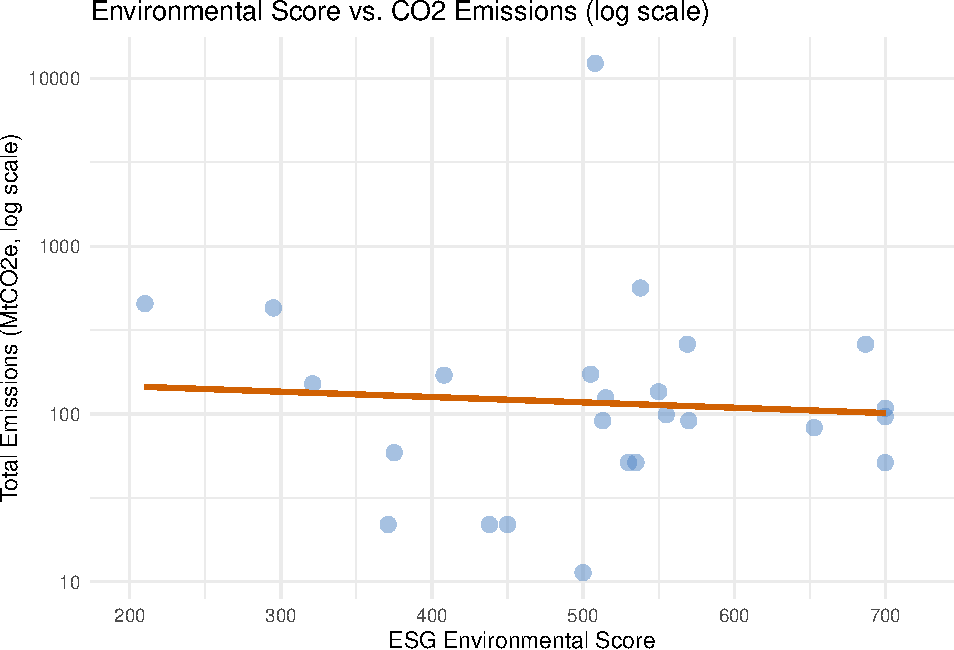
\includegraphics{ESG-code_files/figure-latex/esg-vs-emissions-plot-1.pdf}

\begin{Shaded}
\begin{Highlighting}[]
\NormalTok{matched\_count }\OtherTok{\textless{}{-}} \FunctionTok{sum}\NormalTok{(}\SpecialCharTok{!}\FunctionTok{is.na}\NormalTok{(fuzzy\_merged\_clean}\SpecialCharTok{$}\NormalTok{total\_emissions))}
\NormalTok{unmatched\_count }\OtherTok{\textless{}{-}} \FunctionTok{sum}\NormalTok{(}\FunctionTok{is.na}\NormalTok{(fuzzy\_merged\_clean}\SpecialCharTok{$}\NormalTok{total\_emissions))}
\NormalTok{zero\_count }\OtherTok{\textless{}{-}} \FunctionTok{sum}\NormalTok{(fuzzy\_merged\_clean}\SpecialCharTok{$}\NormalTok{total\_emissions }\SpecialCharTok{==} \DecValTok{0}\NormalTok{, }\AttributeTok{na.rm =} \ConstantTok{TRUE}\NormalTok{)}

\FunctionTok{cat}\NormalTok{(}\StringTok{"Matched records:"}\NormalTok{, matched\_count, }\StringTok{"}\SpecialCharTok{\textbackslash{}n}\StringTok{"}\NormalTok{)}
\end{Highlighting}
\end{Shaded}

\begin{verbatim}
## Matched records: 25
\end{verbatim}

\begin{Shaded}
\begin{Highlighting}[]
\FunctionTok{cat}\NormalTok{(}\StringTok{"Unmatched (NA) records:"}\NormalTok{, unmatched\_count, }\StringTok{"}\SpecialCharTok{\textbackslash{}n}\StringTok{"}\NormalTok{)}
\end{Highlighting}
\end{Shaded}

\begin{verbatim}
## Unmatched (NA) records: 697
\end{verbatim}

\begin{Shaded}
\begin{Highlighting}[]
\FunctionTok{cat}\NormalTok{(}\StringTok{"Zero emission records:"}\NormalTok{, zero\_count, }\StringTok{"}\SpecialCharTok{\textbackslash{}n}\StringTok{"}\NormalTok{)}
\end{Highlighting}
\end{Shaded}

\begin{verbatim}
## Zero emission records: 0
\end{verbatim}

Only 25 firms successfully matched. Most others had unmatched or missing
emissions data. Skewness in CO₂ emissions due to one or two large
emitters (max \textgreater{} 12,000 MtCO₂e).

\hypertarget{correlation-and-linear-regression}{%
\subsection{4. Correlation and Linear
Regression}\label{correlation-and-linear-regression}}

\begin{Shaded}
\begin{Highlighting}[]
\FunctionTok{cor.test}\NormalTok{(fuzzy\_merged\_clean}\SpecialCharTok{$}\NormalTok{environment\_score, }\FunctionTok{log10}\NormalTok{(fuzzy\_merged\_clean}\SpecialCharTok{$}\NormalTok{total\_emissions))}
\end{Highlighting}
\end{Shaded}

\begin{verbatim}
## 
##  Pearson's product-moment correlation
## 
## data:  fuzzy_merged_clean$environment_score and log10(fuzzy_merged_clean$total_emissions)
## t = -0.3285, df = 23, p-value = 0.7455
## alternative hypothesis: true correlation is not equal to 0
## 95 percent confidence interval:
##  -0.4512816  0.3358637
## sample estimates:
##         cor 
## -0.06833607
\end{verbatim}

\begin{Shaded}
\begin{Highlighting}[]
\NormalTok{model }\OtherTok{\textless{}{-}} \FunctionTok{lm}\NormalTok{(}\FunctionTok{log10}\NormalTok{(total\_emissions) }\SpecialCharTok{\textasciitilde{}}\NormalTok{ environment\_score, }\AttributeTok{data =}\NormalTok{ fuzzy\_merged\_clean)}
\FunctionTok{summary}\NormalTok{(model)}
\end{Highlighting}
\end{Shaded}

\begin{verbatim}
## 
## Call:
## lm(formula = log10(total_emissions) ~ environment_score, data = fuzzy_merged_clean)
## 
## Residuals:
##     Min      1Q  Median      3Q     Max 
## -1.0146 -0.3397 -0.0211  0.1693  2.0229 
## 
## Coefficients:
##                     Estimate Std. Error t value Pr(>|t|)    
## (Intercept)        2.2281071  0.5062726   4.401 0.000207 ***
## environment_score -0.0003177  0.0009673  -0.328 0.745509    
## ---
## Signif. codes:  0 '***' 0.001 '**' 0.01 '*' 0.05 '.' 0.1 ' ' 1
## 
## Residual standard error: 0.6128 on 23 degrees of freedom
##   (697 observations deleted due to missingness)
## Multiple R-squared:  0.00467,    Adjusted R-squared:  -0.03861 
## F-statistic: 0.1079 on 1 and 23 DF,  p-value: 0.7455
\end{verbatim}

Environmental Score vs.~CO₂ Emissions (log₁₀) Pearson correlation: r =
-0.068, p = 0.75 Regression coefficient: -0.00032 (not significant, p =
0.75) R² = 0.005 → No significant relationship between environmental
score and emissions.

\begin{Shaded}
\begin{Highlighting}[]
\NormalTok{model\_ln }\OtherTok{\textless{}{-}} \FunctionTok{lm}\NormalTok{(}\FunctionTok{log}\NormalTok{(total\_emissions) }\SpecialCharTok{\textasciitilde{}}\NormalTok{ environment\_score, }\AttributeTok{data =}\NormalTok{ fuzzy\_merged\_clean)}
\FunctionTok{summary}\NormalTok{(model\_ln)}
\end{Highlighting}
\end{Shaded}

\begin{verbatim}
## 
## Call:
## lm(formula = log(total_emissions) ~ environment_score, data = fuzzy_merged_clean)
## 
## Residuals:
##     Min      1Q  Median      3Q     Max 
## -2.3361 -0.7821 -0.0486  0.3898  4.6578 
## 
## Coefficients:
##                     Estimate Std. Error t value Pr(>|t|)    
## (Intercept)        5.1304061  1.1657357   4.401 0.000207 ***
## environment_score -0.0007316  0.0022272  -0.328 0.745509    
## ---
## Signif. codes:  0 '***' 0.001 '**' 0.01 '*' 0.05 '.' 0.1 ' ' 1
## 
## Residual standard error: 1.411 on 23 degrees of freedom
##   (697 observations deleted due to missingness)
## Multiple R-squared:  0.00467,    Adjusted R-squared:  -0.03861 
## F-statistic: 0.1079 on 1 and 23 DF,  p-value: 0.7455
\end{verbatim}

Coefficient (slope): -0.00073 p-value: 0.75 R² = 0.005 Conclusion: ESG
scores in this dataset appear poorly aligned with actual emissions. This
raises concerns about greenwashing and highlights the need for better
ESG data transparency.

\begin{Shaded}
\begin{Highlighting}[]
\NormalTok{model\_log2 }\OtherTok{\textless{}{-}} \FunctionTok{lm}\NormalTok{(}\FunctionTok{log2}\NormalTok{(total\_emissions) }\SpecialCharTok{\textasciitilde{}}\NormalTok{ environment\_score, }\AttributeTok{data =}\NormalTok{ fuzzy\_merged\_clean)}
\FunctionTok{summary}\NormalTok{(model\_log2)}
\end{Highlighting}
\end{Shaded}

\begin{verbatim}
## 
## Call:
## lm(formula = log2(total_emissions) ~ environment_score, data = fuzzy_merged_clean)
## 
## Residuals:
##     Min      1Q  Median      3Q     Max 
## -3.3703 -1.1283 -0.0701  0.5624  6.7198 
## 
## Coefficients:
##                    Estimate Std. Error t value Pr(>|t|)    
## (Intercept)        7.401611   1.681801   4.401 0.000207 ***
## environment_score -0.001056   0.003213  -0.328 0.745509    
## ---
## Signif. codes:  0 '***' 0.001 '**' 0.01 '*' 0.05 '.' 0.1 ' ' 1
## 
## Residual standard error: 2.036 on 23 degrees of freedom
##   (697 observations deleted due to missingness)
## Multiple R-squared:  0.00467,    Adjusted R-squared:  -0.03861 
## F-statistic: 0.1079 on 1 and 23 DF,  p-value: 0.7455
\end{verbatim}

Coefficient (slope): --0.00106 p-value: 0.75 R² = 0.005 Conclusion: The
regression shows no statistically significant relationship between a
company's environmental score and its log₂ emissions. The near-zero R²
indicates that ESG scores explain virtually none of the variation in
actual emissions. This further supports the concern that current ESG
ratings may not reflect real environmental performance.

\begin{Shaded}
\begin{Highlighting}[]
\FunctionTok{summary}\NormalTok{(}\FunctionTok{lm}\NormalTok{(}\FunctionTok{log10}\NormalTok{(total\_emissions) }\SpecialCharTok{\textasciitilde{}}\NormalTok{ social\_score, }\AttributeTok{data =}\NormalTok{ fuzzy\_merged\_clean))}
\end{Highlighting}
\end{Shaded}

\begin{verbatim}
## 
## Call:
## lm(formula = log10(total_emissions) ~ social_score, data = fuzzy_merged_clean)
## 
## Residuals:
##      Min       1Q   Median       3Q      Max 
## -1.03935 -0.37290 -0.01435  0.14462  2.01932 
## 
## Coefficients:
##                Estimate Std. Error t value Pr(>|t|)    
## (Intercept)   2.3486829  0.4346626   5.403 1.72e-05 ***
## social_score -0.0008489  0.0012565  -0.676    0.506    
## ---
## Signif. codes:  0 '***' 0.001 '**' 0.01 '*' 0.05 '.' 0.1 ' ' 1
## 
## Residual standard error: 0.6082 on 23 degrees of freedom
##   (697 observations deleted due to missingness)
## Multiple R-squared:  0.01946,    Adjusted R-squared:  -0.02317 
## F-statistic: 0.4565 on 1 and 23 DF,  p-value: 0.506
\end{verbatim}

Coefficient: --0.00085 p-value: 0.51 R² = 0.019 Conclusion: There is no
statistically significant relationship between social scores and CO₂
emissions. The extremely low R² indicates that social scores explain
less than 2\% of emission variation. This suggests social scores may
capture other aspects of ESG performance but not climate impact.

\begin{Shaded}
\begin{Highlighting}[]
\FunctionTok{summary}\NormalTok{(}\FunctionTok{lm}\NormalTok{(}\FunctionTok{log10}\NormalTok{(total\_emissions) }\SpecialCharTok{\textasciitilde{}}\NormalTok{ governance\_score, }\AttributeTok{data =}\NormalTok{ fuzzy\_merged\_clean))}
\end{Highlighting}
\end{Shaded}

\begin{verbatim}
## 
## Call:
## lm(formula = log10(total_emissions) ~ governance_score, data = fuzzy_merged_clean)
## 
## Residuals:
##     Min      1Q  Median      3Q     Max 
## -0.8477 -0.2547 -0.1389  0.1813  1.9165 
## 
## Coefficients:
##                  Estimate Std. Error t value Pr(>|t|)  
## (Intercept)      1.190878   0.569581   2.091   0.0478 *
## governance_score 0.003168   0.002017   1.571   0.1298  
## ---
## Signif. codes:  0 '***' 0.001 '**' 0.01 '*' 0.05 '.' 0.1 ' ' 1
## 
## Residual standard error: 0.5837 on 23 degrees of freedom
##   (697 observations deleted due to missingness)
## Multiple R-squared:  0.09692,    Adjusted R-squared:  0.05765 
## F-statistic: 2.468 on 1 and 23 DF,  p-value: 0.1298
\end{verbatim}

Coefficient: +0.00317 p-value: 0.13 R² = 0.097 Conclusion: Although not
statistically significant at the 5\% level, the governance score shows a
slight positive correlation with emissions. This could reflect the fact
that larger, more bureaucratic firms may have better governance ratings
but also produce more emissions. However, the low R² still indicates
that governance scores explain little of the emissions variance.

\hypertarget{loess-smoother}{%
\subsection{5. LOESS Smoother}\label{loess-smoother}}

\begin{Shaded}
\begin{Highlighting}[]
\FunctionTok{library}\NormalTok{(ggplot2)}
\FunctionTok{ggplot}\NormalTok{(fuzzy\_merged\_clean, }\FunctionTok{aes}\NormalTok{(}\AttributeTok{x =}\NormalTok{ environment\_score, }\AttributeTok{y =} \FunctionTok{log10}\NormalTok{(total\_emissions))) }\SpecialCharTok{+}
  \FunctionTok{geom\_point}\NormalTok{(}\AttributeTok{alpha =} \FloatTok{0.4}\NormalTok{, }\AttributeTok{size =} \DecValTok{2}\NormalTok{) }\SpecialCharTok{+}
  \FunctionTok{geom\_smooth}\NormalTok{(}\AttributeTok{method =} \StringTok{"loess"}\NormalTok{, }\AttributeTok{color =} \StringTok{"red"}\NormalTok{, }\AttributeTok{se =} \ConstantTok{FALSE}\NormalTok{, }\AttributeTok{span =} \FloatTok{0.75}\NormalTok{) }\SpecialCharTok{+}
  \FunctionTok{labs}\NormalTok{(}
    \AttributeTok{title =} \StringTok{"ESG Environmental Score vs. CO2 Emissions"}\NormalTok{,}
    \AttributeTok{x =} \StringTok{"Environmental Score"}\NormalTok{,}
    \AttributeTok{y =} \StringTok{"Log10 of CO2 Emissions (MtCO2e)"}
\NormalTok{  ) }\SpecialCharTok{+}
  \FunctionTok{theme\_minimal}\NormalTok{(}\AttributeTok{base\_size =} \DecValTok{14}\NormalTok{)}\SpecialCharTok{+}
  \FunctionTok{theme}\NormalTok{(}
    \AttributeTok{panel.grid.major =} \FunctionTok{element\_line}\NormalTok{(}\AttributeTok{color =} \StringTok{"gray90"}\NormalTok{),}
    \AttributeTok{panel.grid.minor =} \FunctionTok{element\_blank}\NormalTok{()}
\NormalTok{  )}
\end{Highlighting}
\end{Shaded}

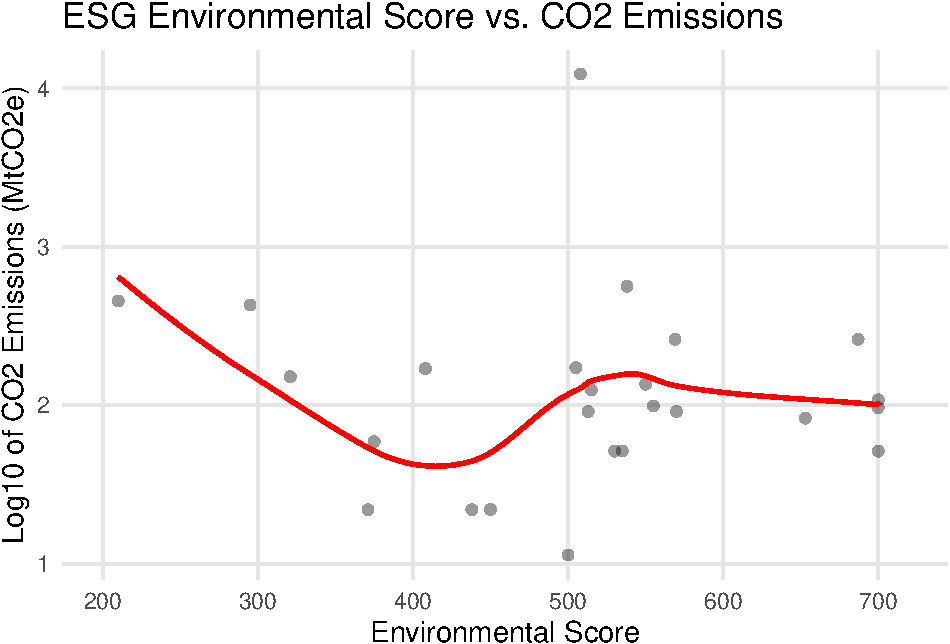
\includegraphics{ESG-code_files/figure-latex/loess-plot-1.pdf} While the
correlation is weak and statistically insignificant, the nonlinear
pattern suggests an interesting shape: Firms with lower environmental
scores tend to have higher emissions, aligning with expectations.
However, for firms with moderate to high scores (400--600), emissions do
not consistently decline --- in fact, emissions slightly increase and
then flatten out. \#\# 6. Diagnostics

\begin{Shaded}
\begin{Highlighting}[]
\FunctionTok{cor.test}\NormalTok{(fuzzy\_merged\_clean}\SpecialCharTok{$}\NormalTok{environment\_score, }
         \FunctionTok{log}\NormalTok{(fuzzy\_merged\_clean}\SpecialCharTok{$}\NormalTok{total\_emissions), }
         \AttributeTok{method =} \StringTok{"pearson"}\NormalTok{)}
\end{Highlighting}
\end{Shaded}

\begin{verbatim}
## 
##  Pearson's product-moment correlation
## 
## data:  fuzzy_merged_clean$environment_score and log(fuzzy_merged_clean$total_emissions)
## t = -0.3285, df = 23, p-value = 0.7455
## alternative hypothesis: true correlation is not equal to 0
## 95 percent confidence interval:
##  -0.4512816  0.3358637
## sample estimates:
##         cor 
## -0.06833607
\end{verbatim}

\begin{Shaded}
\begin{Highlighting}[]
\FunctionTok{par}\NormalTok{(}\AttributeTok{mfrow =} \FunctionTok{c}\NormalTok{(}\DecValTok{2}\NormalTok{, }\DecValTok{2}\NormalTok{))}
\FunctionTok{plot}\NormalTok{(model\_ln)}
\end{Highlighting}
\end{Shaded}

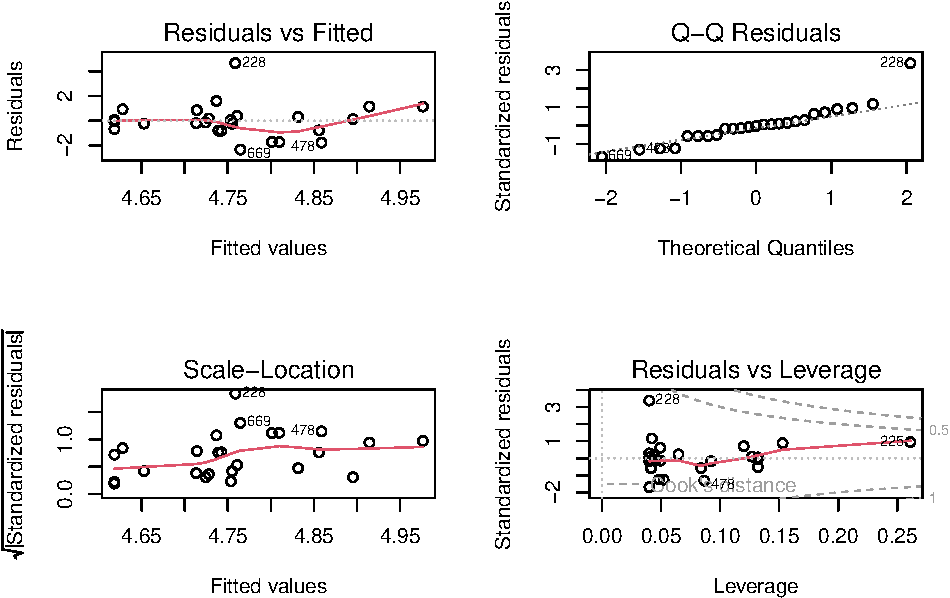
\includegraphics{ESG-code_files/figure-latex/diagnostics-1.pdf}
Regression Diagnostics: The residual plots suggest that while most
assumptions are reasonably met, there are a few mild deviations from
normality (Q-Q plot) and potential mild heteroskedasticity
(Scale-Location). A few influential observations (e.g., point 228) have
moderate leverage but do not exceed Cook's threshold. Overall, the
linear model remains interpretable, though results should be interpreted
with caution given the weak R² and small sample size.

\hypertarget{summary-of-results}{%
\subsection{7. Summary of Results}\label{summary-of-results}}

• Slope: -0.0003 → A 1-point increase in environmental score correlates
with a \textasciitilde0.03\% decrease in CO₂ emissions --- though the
effect is statistically insignificant. • p-value: 0.7455 → No evidence
of a meaningful relationship between environmental score and emissions.
• R²: \textasciitilde0.005 → ESG score explains less than 1\% of the
variance in carbon emissions.

Despite ESG scores being widely used to evaluate corporate
responsibility, these results suggest that high scores do not reliably
correspond to low carbon output --- at least not in this subset of
companies with emissions data. The LOESS and residual plots further
support this conclusion, showing high variance and weak fit.

\hypertarget{conclusion}{%
\subsection{8. Conclusion}\label{conclusion}}

This analysis finds \textbf{no statistically significant relationship}
between ESG environmental scores and actual carbon emissions among
companies in this matched sample. While ESG ratings may capture
qualitative policies, intentions, or disclosures, they do not appear to
reflect real environmental performance --- especially in high-emitting
sectors.

For investors, regulators, and ESG-focused institutions, this calls for
greater scrutiny into how ESG metrics are constructed, and whether they
can be relied upon as indicators of measurable impact. This case study
highlights the need for stronger alignment between ESG scoring
frameworks and independently verified environmental outcomes.

\hypertarget{appendix}{%
\subsection{9. Appendix}\label{appendix}}

\begin{Shaded}
\begin{Highlighting}[]
\FunctionTok{summary}\NormalTok{(emissions)}
\end{Highlighting}
\end{Shaded}

\begin{verbatim}
##       year      parent_entity      parent_type         commodity        
##  Min.   :1854   Length:12551       Length:12551       Length:12551      
##  1st Qu.:1973   Class :character   Class :character   Class :character  
##  Median :1994   Mode  :character   Mode  :character   Mode  :character  
##  Mean   :1987                                                           
##  3rd Qu.:2009                                                           
##  Max.   :2022                                                           
##  production_value    production_unit    total_emissions_MtCO2e
##  Min.   :    0.004   Length:12551       Min.   :   0.000      
##  1st Qu.:   10.601   Class :character   1st Qu.:   8.785      
##  Median :   63.204   Mode  :character   Median :  33.059      
##  Mean   :  412.677                      Mean   : 113.206      
##  3rd Qu.:  320.665                      3rd Qu.: 102.155      
##  Max.   :27192.000                      Max.   :8646.906
\end{verbatim}

\begin{Shaded}
\begin{Highlighting}[]
\FunctionTok{glimpse}\NormalTok{(emissions)}
\end{Highlighting}
\end{Shaded}

\begin{verbatim}
## Rows: 12,551
## Columns: 7
## $ year                   <dbl> 1962, 1962, 1963, 1963, 1964, 1964, 1965, 1965,~
## $ parent_entity          <chr> "Abu Dhabi National Oil Company", "Abu Dhabi Na~
## $ parent_type            <chr> "State-owned Entity", "State-owned Entity", "St~
## $ commodity              <chr> "Oil & NGL", "Natural Gas", "Oil & NGL", "Natur~
## $ production_value       <dbl> 0.91250, 1.84325, 1.82500, 4.42380, 7.30000, 17~
## $ production_unit        <chr> "Million bbl/yr", "Bcf/yr", "Million bbl/yr", "~
## $ total_emissions_MtCO2e <dbl> 0.3638848, 0.1343552, 0.7277697, 0.3224525, 2.9~
\end{verbatim}

\begin{Shaded}
\begin{Highlighting}[]
\FunctionTok{glimpse}\NormalTok{(esg\_data) }
\end{Highlighting}
\end{Shaded}

\begin{verbatim}
## Rows: 722
## Columns: 21
## $ ticker               <chr> "dis", "gm", "gww", "mhk", "lyv", "lvs", "clx", "~
## $ name                 <chr> "Walt Disney Co", "General Motors Co", "WW Graing~
## $ currency             <chr> "USD", "USD", "USD", "USD", "USD", "USD", "USD", ~
## $ exchange             <chr> "NEW YORK STOCK EXCHANGE, INC.", "NEW YORK STOCK ~
## $ industry             <chr> "Media", "Automobiles", "Trading Companies and Di~
## $ logo                 <chr> "https://static.finnhub.io/logo/ef50b4a2b263c8472~
## $ weburl               <chr> "https://thewaltdisneycompany.com/", "https://www~
## $ environment_grade    <chr> "A", "A", "B", "A", "BBB", "A", "A", "B", "B", "B~
## $ environment_level    <chr> "High", "High", "Medium", "High", "High", "High",~
## $ social_grade         <chr> "BB", "BB", "BB", "B", "BB", "BB", "BB", "B", "B"~
## $ social_level         <chr> "Medium", "Medium", "Medium", "Medium", "Medium",~
## $ governance_grade     <chr> "BB", "B", "B", "BB", "B", "BB", "BB", "B", "B", ~
## $ governance_level     <chr> "Medium", "Medium", "Medium", "Medium", "Medium",~
## $ environment_score    <dbl> 510, 510, 255, 570, 492, 547, 560, 203, 270, 220,~
## $ social_score         <dbl> 316, 303, 385, 298, 310, 318, 350, 200, 211, 221,~
## $ governance_score     <dbl> 321, 255, 240, 303, 250, 313, 345, 205, 265, 300,~
## $ total_score          <dbl> 1147, 1068, 880, 1171, 1052, 1178, 1255, 608, 746~
## $ last_processing_date <chr> "19-04-2022", "17-04-2022", "19-04-2022", "18-04-~
## $ total_grade          <chr> "BBB", "BBB", "BB", "BBB", "BBB", "BBB", "A", "B"~
## $ total_level          <chr> "High", "High", "Medium", "High", "High", "High",~
## $ cik                  <dbl> 1744489, 1467858, 277135, 851968, 1335258, 130051~
\end{verbatim}

\begin{Shaded}
\begin{Highlighting}[]
\FunctionTok{summary}\NormalTok{(esg\_data)}
\end{Highlighting}
\end{Shaded}

\begin{verbatim}
##     ticker              name             currency           exchange        
##  Length:722         Length:722         Length:722         Length:722        
##  Class :character   Class :character   Class :character   Class :character  
##  Mode  :character   Mode  :character   Mode  :character   Mode  :character  
##                                                                             
##                                                                             
##                                                                             
##    industry             logo              weburl          environment_grade 
##  Length:722         Length:722         Length:722         Length:722        
##  Class :character   Class :character   Class :character   Class :character  
##  Mode  :character   Mode  :character   Mode  :character   Mode  :character  
##                                                                             
##                                                                             
##                                                                             
##  environment_level  social_grade       social_level       governance_grade  
##  Length:722         Length:722         Length:722         Length:722        
##  Class :character   Class :character   Class :character   Class :character  
##  Mode  :character   Mode  :character   Mode  :character   Mode  :character  
##                                                                             
##                                                                             
##                                                                             
##  governance_level   environment_score  social_score   governance_score
##  Length:722         Min.   :200.0     Min.   :160.0   Min.   : 75.0   
##  Class :character   1st Qu.:240.0     1st Qu.:243.0   1st Qu.:235.0   
##  Mode  :character   Median :483.0     Median :302.0   Median :300.0   
##                     Mean   :404.8     Mean   :292.2   Mean   :278.8   
##                     3rd Qu.:518.8     3rd Qu.:322.8   3rd Qu.:310.0   
##                     Max.   :719.0     Max.   :667.0   Max.   :475.0   
##   total_score     last_processing_date total_grade        total_level       
##  Min.   : 600.0   Length:722           Length:722         Length:722        
##  1st Qu.: 763.0   Class :character     Class :character   Class :character  
##  Median :1046.0   Mode  :character     Mode  :character   Mode  :character  
##  Mean   : 975.8                                                             
##  3rd Qu.:1144.0                                                             
##  Max.   :1536.0                                                             
##       cik         
##  Min.   :   1800  
##  1st Qu.: 723157  
##  Median :1046189  
##  Mean   : 989792  
##  3rd Qu.:1470094  
##  Max.   :1914023
\end{verbatim}

\end{document}
